\documentclass{article}
\usepackage{graphicx}
\usepackage{amssymb}
\usepackage{amsmath}
\usepackage{tikz}
\usepackage{url}
\usetikzlibrary{shapes}


\linespread{1.4}

\title{Genome Compression Against a Reference \\
        Project Proposal \\}

\author{\\
        Aniruddha Laud (107635282)\\
        Gaurav Menghani (108266803)\\
        Madhava Keralapura (107710538)\\}


\begin{document}

\maketitle

\clearpage
.
\clearpage

\tableofcontents

\clearpage

\section {Introduction}
TODO
\clearpage

\section {Relevant Work}
TODO
\clearpage

\section {Work Done}

\subsection {Storing the Bit Vectors Efficiently}
TODO and add charts

\clearpage

\subsection {Improving the Variable Integer (VINT) storage}
The DNAZip source code makes heavy use of Variable Integer (VINT) storage, so that they do not have to allocate a fixed
number of bits for each integer value that needs to be written. The reason being, if we are writing very small values, and the data type of our choice is the standard integer, we would be using 32 bits for each value that we write but most of the higher bits in the number would not be set. However, if we choose a small data type like a byte, we would not be able to write values greater than $2^8 - 1$. \\
This is solved by writing 8 bits at a time, of which the MSB is set if there is another block of 8 bits for the number after the current block. Thus, out of the 8 bits, 1 bit is a flag, and the rest 7 come from the number to be written. We realized that this might not be the most efficient way of doing it. A large number of values written as variable integers are small delta values, and writing 8 bits at a time would mean that atleast 8 bits would be written even if the number is very small. \\
The values being written as VINTs during the compression process were written to an auxilliary file. We then tried to compare the space consumed when the size of the VINT word size is varied. 

\begin{figure}[htp]
\centering
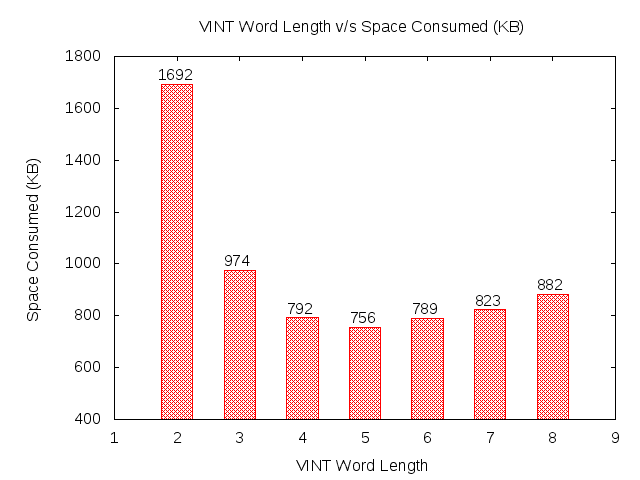
\includegraphics[scale=0.4]{images/VINT.png}
\caption{VINT Word Length v/s Space Consumed (KB)}\label{fig:fs}
\end{figure}
\clearpage
Thus, with the VINT word size as 8, 882 KB of space was being used up for writing VINTs. The optimal VINT word size was found to be 5, which as per experiments would have used up 756 KB of space.\\
\\ 
The actual compression received from this was 129 KB roughly, which was in line with our expectation before this experiment.\\
\clearpage

\subsection {Improving the storing of Insertion/Deletion (INDEL)}
After thorough analysis, we realized that the Insertion/Deletion format in iteself was pretty packed. One optimization possible was to create a Bit Vector for the Insertions and Deletions which were present in dbSNP. This meant that we would not need to store the information for the insertions and deletions which existed in the dbSNP. A bit vector for the insertions / deletions present in dbSNP could be used to encode that information.\\ 
\\
For insertions we noticed that the number of insertions in the Genome which existed in dbSNP were very few. Thus, the bit vector was extremely sparse. (TODO write figures?) \\
\\
For deletions this number was significant but still not large enough. The percentage of deletions in a chromosome which existin dbSNP varies from 5.3\% to 11.68\% (apart from the Mitochondrial DNA, which has only deletion, which does not exist in dbSNP).

\begin{center}
	\begin{tabular}{|p{1in}|p{1in}|}
	\hline
	Chromosome	&		\% of Deletions found in dbSNP \\
	\hline
	1	&		8.54 \\
	\hline
	2	&		8.76 \\
	\hline
	3	&		8.80 \\
	\hline
	4	&	11.67 \\
	\hline
	5	&	10.46 \\
	\hline
	6	&	8.87 \\
	\hline
	7	&	6.90 \\
	\hline
	8	&	9.45 \\
	\hline
	9	&	7.84 \\
	\hline
	10	&	9.40 \\
	\hline
	11	&	10.09 \\
	\hline
	12	&	6.39 \\
	\hline
	13	&	6.70 \\
	\hline
	14	&	9.63 \\
	\hline
	15	&	6.99 \\
	\hline
	16	&	6.74 \\	
	\hline
	17	&	6.50 \\
	\hline	
	18	&	10.61 \\
	\hline	
	19	&	5.30 \\
	\hline
	20	&	13.06 \\	
	\hline
	21	&	10.36 \\
	\hline
	22	&	7.08  \\
	\hline
	Mitochondrial	&	0.0 \\
	\hline
	X	&	7.57 \\
	\hline
	\end{tabular}

\end{center}























We compressed the bit vector using Run-Length Encoding. This gave us a saving of about 10 KB. Using Huffman Encoding gave us a saving of roughly 20 KB. Another 1 KB of compression was squeezed in my noticing that the bit vector was sparser than the SNP bit vector, and a k-mer length of size 7 was the most suitable for this.\\ 
\\
Thus, we only changed the storage for the deletions. The deletions which were present in dbSNP were stored using bitvectors, and compressed using Huffman Encoding with k-mer size as 7.
\clearpage

\section {Results \& Conclusion}
The original DNAZip format was already pretty efficient. However, over the course of project, we have exploited avenues where we could foresee significant compression possible. Towards the end of the project, it became hard to find any further improvements.\\
\\
In all we have compressed James Watson's genome to 3736918 bytes, from the original 4198717 bytes used by the DNAZip format. This is a compression of roughly 10.998\%. \\

TODO: Finish This
\clearpage

\begin{thebibliography}{}

\bibitem{jorde04}
  Jorde, Lynn B. and Wooding, Stephen P.,
  \emph{Genetic variation, classification and race}.
  Nature Genetics 36 (11 Suppl): S28–S33. doi:10.1038/ng1435. PMID 15508000,
  2004

\bibitem{ucschg}
  UCSC Genome Bioinformatics, Human (Homo sapiens) Genome Browser Gateway
  http://genome.ucsc.edu/cgi-bin/hgGateway

\bibitem{ucschg18}
  UCSC Genome Bioinformatics, Human Chromosome (hg18)
  http://hgdownload.cse.ucsc.edu/goldenPath/hg18/chromosomes/

\bibitem{dnazip}
  The DNA Zip Project
  http://www.ics.uci.edu/~dnazip/

\bibitem{dnazip_paper}
  Christley, Scott and Lu, Yiming and Li, Chen and Xie, Xiaohui,
  \emph{Human genomes as email attachments}.

\bibitem{gencompress}
  Chen, Xi and Kwong, Sam and Li, Ming,
  \emph{A Compression Algorithm for DNA Sequences and Its Applications in Genome Comparison}
 
\bibitem{jwseq}
  James Watson's Sequence
  http://jimwatsonsequence.cshl.edu/cgi-perl/gbrowse/jwsequence/

\bibitem{completegenomics}
  Complete Genomics
  http://www.completegenomics.com/ 
\end{thebibliography}

\end{document}
